\documentclass[11pt,a4paper,english]{article}
    \usepackage[latin1]{inputenc}
    \usepackage{amsmath,amsfonts,amssymb}
    \usepackage{enumitem}
    \usepackage{fullpage}
    \usepackage{graphicx}
    \usepackage{tabto}
    \usepackage{etoolbox}
    \usepackage{hyperref}
    \usepackage{minted}
    \usepackage{parskip}
    \usepackage[title]{appendix}
    \graphicspath{ {./} }

    \title{Bayesian Data Analysis - Assignment 4}
    \author{}

    \begin{document}
      \maketitle
      \definecolor{bg}{rgb}{0.95,0.95,0.95}

      We can derive $\sigma$, $\mu$ and $convarience\ matrix$ from the given
      normal distributions of $\alpha \sim N(0, 2^2)$ and $\beta \sim N(10, 10^2)$.

      \begin{minted}[bgcolor=bg,linenos,fontsize=\small,autogobble]{python}
        sigma_a = 2
        sigma_b = 10
        mu_a = 0
        mu_b = 10
        cor = 0.5
        cov_matrix = np.array([
            [sigma_a**2,                cor * sigma_a * sigma_b],
            [cor * sigma_a * sigma_b,   sigma_b**2]]
        )
      \end{minted}

      This initialization allows us to calculate and plot \textbf{prior distribution}:

      \begin{minted}[bgcolor=bg,linenos,fontsize=\small,autogobble]{python}
        # create a grid and it's points using x and y ranges
        alpha, beta = np.meshgrid(np.linspace(-4, 4, 100), np.linspace(-10, 30, 100))
        points = np.dstack((alpha, beta))

        # prior distribution
        mean = np.array([mu_a, mu_b])
        prior_multivar_nor = stats.multivariate_normal(mean, cov_matrix)
        prior = prior_multivar_nor.pdf(points)
        plt.contourf(alpha, beta, prior)
      \end{minted}

      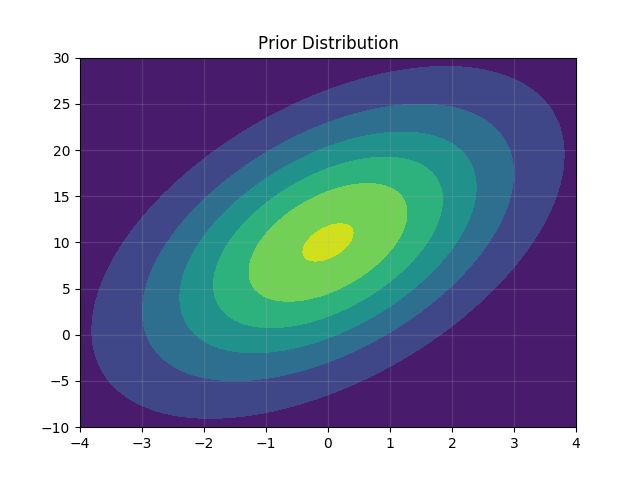
\includegraphics[width=9cm]{1_prior_distribution.png}

      To calculate the \textbf{likelihood} though, we have to take into consideration the
      data from the book that indicates the values of $doses$, $deaths$ and $number\ of\ animals$; and
      use the \href{https://github.com/avehtari/BDA_course_Aalto/blob/master/exercises/additional_files/bioassaylp.py}{bioassaylp}
      function:
      \begin{minted}[bgcolor=bg,linenos,fontsize=\small,autogobble]{python}
        doses = np.array([-0.86, -0.3, -0.05, 0.72])
        deaths = np.array([0, 1, 3, 5])
        number_of_animals = np.array([5, 5, 5, 5])

        likelihood = bioassaylp(alpha, beta, doses, deaths, number_of_animals)
        plt.contourf(alpha, beta, np.exp(likelihood))
      \end{minted}

      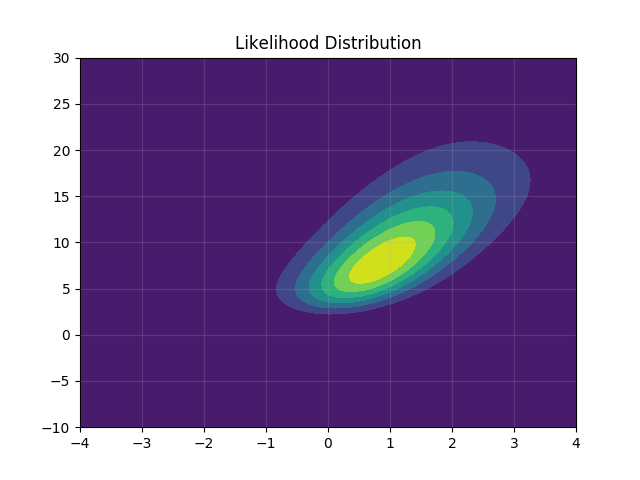
\includegraphics[width=10cm]{2_likelihood_distribution.png}

      Calculating \textbf{posterior} is straight forward, we have to just multiply the likelihood
      with prior:
      \begin{minted}[bgcolor=bg,linenos,fontsize=\small,autogobble]{python}
        posterior = prior * np.exp(likelihood)
        plt.contourf(alpha, beta, posterior)
      \end{minted}

      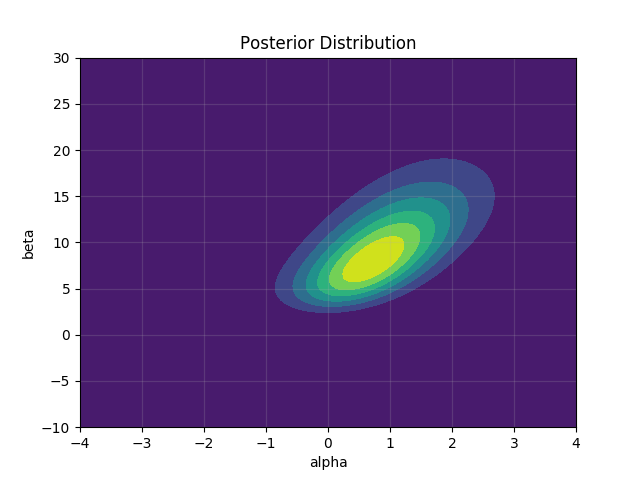
\includegraphics[width=10cm]{3_posterior_distribution.png}

      Using the prior distribution we can \textbf{draw a sample with a size = 10000}:
      \begin{minted}[bgcolor=bg,linenos,fontsize=\small,autogobble]{python}
        samples_from_prior = prior_multivar_nor.rvs(10000)
      \end{minted}

      We can then compute \textbf{the importance ratios for each draw} like:
      \begin{minted}[bgcolor=bg,linenos,fontsize=\small,autogobble]{bash}
        logit = 1 / (
            1 + np.exp(
                -(samples_from_prior[:, 0, None] + samples_from_prior[:, 1, None] * doses)
            )
        )

        weights_of_likelihood = np.prod(
            logit**deaths * (1 - logit)**(number_of_animals - deaths),
            axis=1
        )
        print('Shape of the weights of the likelihood: ', weights_of_likelihood.shape)
      \end{minted}

      Consequently, \textbf{the effective sample size $S_{eff}$} would be calculated as:
      \begin{minted}[bgcolor=bg,linenos,fontsize=\small,autogobble]{bash}
        weights_norm = (weights_of_likelihood) / np.sum(weights_of_likelihood)
        S_eff = 1 / np.sum(weights_norm**2)
        print('The effective sample size: ', round(S_eff, 4))
      \end{minted}

      Which outputs:
      \begin{minted}[bgcolor=bg,linenos,fontsize=\small,autogobble]{bash}
        $ The effective sample size:  2725.6818
      \end{minted}

      We can then easily compute the \textbf{posterior mean} using importance sampling:
      \begin{minted}[bgcolor=bg,linenos,fontsize=\small,autogobble]{bash}
        mean_posterior = sum(
          weights_of_likelihood[ : , None] * samples_from_prior
        ) / sum(weights_of_likelihood)
        print('The posterior mean of alpha : ', round(mean_posterior[0], 4))
        print('The posterior mean of beta  : ', round(mean_posterior[1], 4))
      \end{minted}

      Which are:
      \begin{minted}[bgcolor=bg,linenos,fontsize=\small,autogobble]{bash}
        $ The posterior mean of alpha :  0.9786
        $ The posterior mean of beta  :  10.4321
      \end{minted}

      Using importance resampling we can obtain a \textbf{posterior sample of size 1000} of alpha and beta:
      \begin{minted}[bgcolor=bg,linenos,fontsize=\small,autogobble]{bash}
        gen_nums = np.random.RandomState(0).choice(
          a=10000, size=1000, replace=False, p=weights_norm
        )
        resamples = samples_from_prior[gen_nums]
        print('The posterior mean of alpha: ', round(np.mean(resamples[:, 0]), 4))
        print('The posterior mean of beta: ', round(np.mean(resamples[:, 1]), 4))
      \end{minted}

      Which are:
      \begin{minted}[bgcolor=bg,linenos,fontsize=\small,autogobble]{bash}
        $ The posterior mean of alpha:  0.9359
        $ The posterior mean of beta:  10.3614
      \end{minted}

      If we combine these two we will have $\alpha =$ \textbf{[0.9359, 0.9786]} and
      $beta =$ \textbf{[10.4321, 10.3614]}.

      Finally, we can \textbf{plot a scatterplot of the obtained posterior sample} from importance resampling
      and compare it to the heatmap:

      \begin{minted}[bgcolor=bg,linenos,fontsize=\small,autogobble]{bash}
        fig, axes = plt.subplots(1, 3, figsize=(16, 5))
        axes[0].scatter(resamples[:, 0], resamples[:, 1], 10)
        axes[1].grid(linewidth=0.9, alpha=0.2)
        axes[2].contourf(alpha, beta, posterior)
        axes[2].scatter(resamples[:, 0], resamples[:, 1], 10, alpha=0.3, color='w')
      \end{minted}

      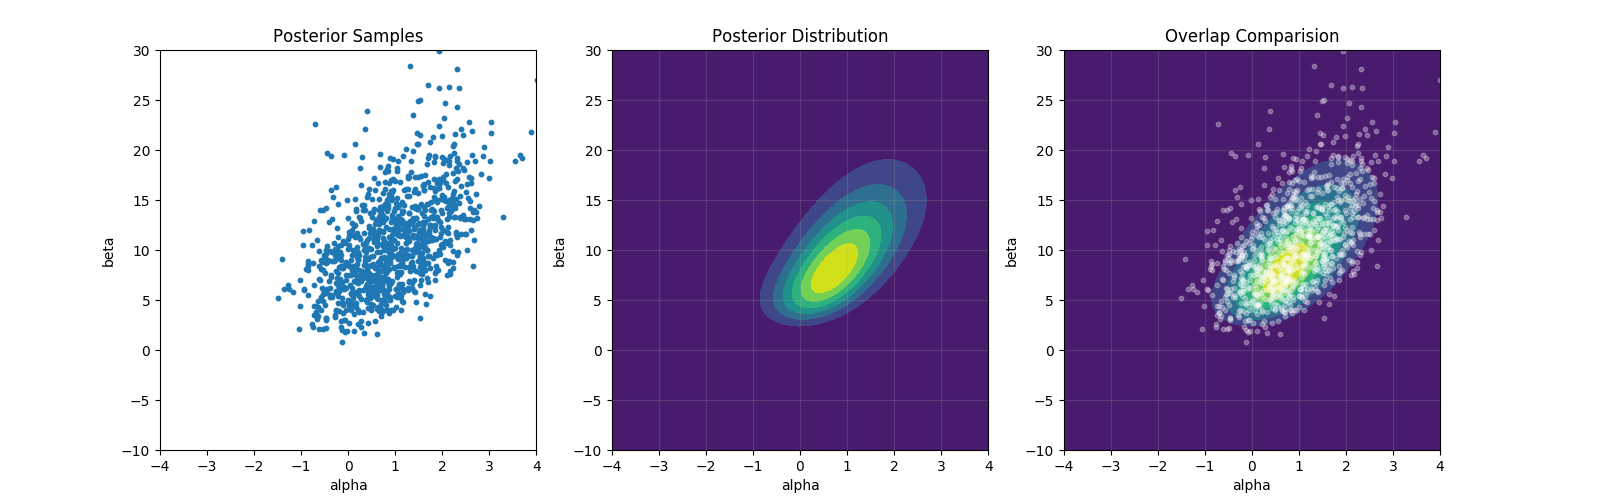
\includegraphics[width=17.7cm]{4_posterior_comparision.png}

      The \textbf{estimate $p(beta > 0 | x, n, y)$ probability} can be calculated as:
      \begin{minted}[bgcolor=bg,linenos,fontsize=\small,autogobble]{bash}
        beta_resample = resamples[:, 1]
        alpha_resample = resamples[:,0]
        pos = beta_resample > 0
        probab_drug_harmful = (beta_resample[pos].size/(beta_resample.size))
        print('Probability of the drug being harmful: ', round(probab_drug_harmful, 3))
      \end{minted}

      \begin{minted}[bgcolor=bg,linenos,fontsize=\small,autogobble]{bash}
        $ Probability of the drug being harmful is very close to:  1
      \end{minted}

      And the \textbf{histogram} can be plotted like:

      \begin{minted}[bgcolor=bg,linenos,fontsize=\small,autogobble]{bash}
        sample_ld50 = -alpha_resample[pos]/beta_resample[pos]
        y_range = np.arange(-0.45, 0.45, 0.01)
        plt.hist(sample_ld50, y_range, ec='white', alpha=0.7)
      \end{minted}
      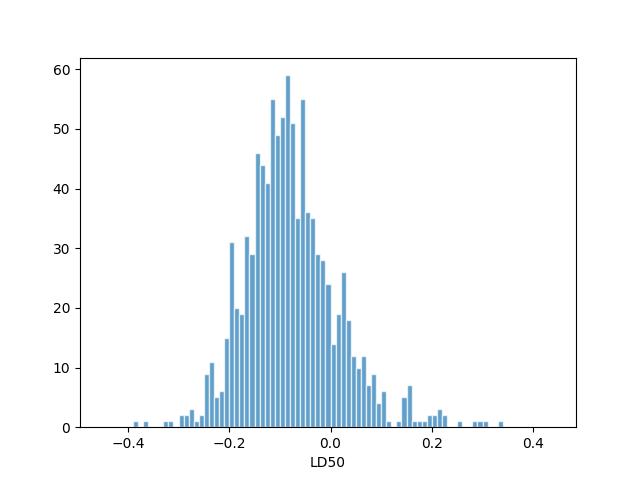
\includegraphics[width=10cm]{5_histogram.png}

      \begin{appendices}
        \section{Source code}
        \begin{minted}[bgcolor=bg,linenos,fontsize=\small,autogobble]{python}
          import matplotlib
          matplotlib.use('TkAgg')
          import matplotlib.pyplot as plt
          from mpl_toolkits.mplot3d import Axes3D
          from scipy import stats
          import numpy as np

          def bioassaylp(a, b, x, y, n):
              # last axis for the data points
              a = np.expand_dims(a, axis=-1)
              b = np.expand_dims(b, axis=-1)
              # these help using chain rule in derivation
              t = a + b*x
              et = np.exp(t)
              z = et/(1.+et)
              # negative log posterior (error function to be minimized)
              lp = np.sum(y*np.log(z)+ (n-y)*np.log(1.0-z), axis=-1)
              return lp

          # Init all the params based on the description
          sigma_a = 2
          sigma_b = 10
          mu_a = 0
          mu_b = 10
          cor = 0.5
          cov_matrix = np.array([
            [sigma_a**2,                cor * sigma_a * sigma_b],
            [cor * sigma_a * sigma_b,   sigma_b**2]]
          )

          # create a grid and it's points using x and y ranges
          alpha, beta = np.meshgrid(np.linspace(-4, 4, 100), np.linspace(-10, 30, 100))
          points = np.dstack((alpha, beta))

          # prior distribution
          mean = np.array([mu_a, mu_b])
          prior_multivar_nor = stats.multivariate_normal(mean, cov_matrix)
          prior = prior_multivar_nor.pdf(points)

          plt.contourf(alpha, beta, prior)
          plt.title('Prior Distribution')
          plt.grid(linewidth=0.9, alpha=0.2)
          plt.savefig('./ex4/report/1_prior_distribution.png')
          plt.figure()

          # likelihood
          doses = np.array([-0.86, -0.3, -0.05, 0.72])
          deaths = np.array([0, 1, 3, 5])
          number_of_animals = np.array([5, 5, 5, 5])

          likelihood = bioassaylp(alpha, beta, doses, deaths, number_of_animals)
          plt.contourf(alpha, beta, np.exp(likelihood))
          plt.title('Likelihood Distribution')
          plt.grid(linewidth=0.9, alpha=0.2)
          plt.savefig('./ex4/report/2_likelihood_distribution.png')
          plt.figure()

          '''
          1. Calculate the posterior density in a grid of points around the prior
          (alpha: 0 +- 4, beta: 10 +- 20) and plot a heatmap of the density.
          '''
          posterior = prior * np.exp(likelihood)
          plt.contourf(alpha, beta, posterior)
          plt.xlabel('alpha')
          plt.ylabel('beta')
          plt.title('Posterior Distribution')
          plt.grid(linewidth=0.9, alpha=0.2)
          plt.savefig('./ex4/report/3_posterior_distribution.png')
          plt.figure()

          '''
          2. Sample draws of alpha and beta from the prior distribution.
          '''
          samples_from_prior = prior_multivar_nor.rvs(10000)
          print('Shape of the samples from prior: ', samples_from_prior.shape)

          '''
          3. Compute the importance ratios for each draw (target distribution is the posterior).
          '''
          logit = 1 / (
              1 + np.exp(
                  -(samples_from_prior[:, 0, None] + samples_from_prior[:, 1, None] * doses)
              )
          )

          weights_of_likelihood = np.prod(
              logit**deaths * (1 - logit)**(number_of_animals - deaths),
              axis=1
          )
          print('Shape of the weights of the likelihood: ', weights_of_likelihood.shape)

          '''
          4. Using the importance ratios, compute the effective sample size Seff and report it.
          If Seff is less than 1000, repeat the importance sampling with more draws.
          '''
          weights_norm = (weights_of_likelihood) / np.sum(weights_of_likelihood)
          S_eff = 1 / np.sum(weights_norm**2)
          print('The effective sample size: ', round(S_eff, 4))

          '''
          5. Compute the posterior mean using importance sampling and report it.
          '''
          mean_posterior = sum(
            weights_of_likelihood[ : , None] * samples_from_prior
            ) / sum(weights_of_likelihood)
          print('The posterior mean of alpha : ', round(mean_posterior[0], 4))
          print('The posterior mean of beta  : ', round(mean_posterior[1], 4))

          '''
          6. Use importance resampling to obtain a posterior sample of size 1000
            of alpha and beta.
          '''
          gen_nums = np.random.RandomState(0).choice(
            a=10000, size=1000, replace=False, p=weights_norm
          )
          resamples = samples_from_prior[gen_nums]
          print('Mean alpha: ', round(np.mean(resamples[:, 0]), 4))
          print('Mean beta: ', round(np.mean(resamples[:, 1]), 4))

          '''
          7. Using the posterior sample obtained via importance resampling:
              7.1 Plot a scatterplot of the obtained posterior sample and compare that to
                  the heatmap plotted earlier.
          '''
          fig, axes = plt.subplots(1, 3, figsize=(16, 5))
          axes[0].set_xlim([-4, 4])
          axes[0].set_ylim([-10, 30])
          axes[0].set_xlabel('alpha')
          axes[0].set_ylabel('beta')
          axes[0].set_title('Posterior Samples')
          axes[0].scatter(resamples[:, 0], resamples[:, 1], 10)

          axes[1].set_xlim([-4, 4])
          axes[1].set_ylim([-10, 30])
          axes[1].set_xlabel('alpha')
          axes[1].set_ylabel('beta')
          axes[1].set_title('Posterior Distribution')
          axes[1].contourf(alpha, beta, posterior)
          axes[1].grid(linewidth=0.9, alpha=0.2)

          axes[2].set_xlim([-4, 4])
          axes[2].set_ylim([-10, 30])
          axes[2].set_xlabel('alpha')
          axes[2].set_ylabel('beta')
          axes[2].set_title('Overlap Comparision')
          axes[2].contourf(alpha, beta, posterior)
          axes[2].scatter(resamples[:, 0], resamples[:, 1], 10, alpha=0.3, color='w')
          axes[2].grid(linewidth=0.9, alpha=0.2)

          plt.subplots_adjust(left=0.1, right=0.9, top=0.9, bottom=0.1)
          plt.savefig('./ex4/report/4_posterior_comparision.png')
          plt.figure()

          '''
              7.2 Report an estimate for p(beta > 0|x, n, y), that is, the
              probability that the drug is harmful.
          '''
          beta_resample = resamples[:, 1]
          alpha_resample = resamples[:,0]
          pos = beta_resample > 0
          probab_drug_harmful = (beta_resample[pos].size/(beta_resample.size))
          print('Probability of the drug being harmful: ', round(probab_drug_harmful, 3))

          '''
              7.3 Draw a histogram of the draws from the posterior distribution of the LD50
                  conditional on beta > 0 (see Figure 3.4).
          '''
          sample_ld50 = -alpha_resample[pos]/beta_resample[pos]
          y_range = np.arange(-0.45, 0.45, 0.01)
          plt.hist(sample_ld50, y_range, ec='white', alpha=0.7)

          plt.xlabel('LD50')
          plt.savefig('./ex4/report/5_histogram.png')
          plt.figure()
        \end{minted}
      \end{appendices}
  \end{document}
